\documentclass{beamer}
\usepackage[normalem]{ulem}
\usepackage{graphicx}

\usetheme{metropolis}

%Information to be included in the title page:
\title{SwarmAvg - A Novel Approach to Fully Distributed Machine Learning}
\author{Josh Pattman}
\institute{University Of Southampton}
\date{May 2023}
\graphicspath{{plots}}

\begin{document}
	\frame{\titlepage}
	
	\section{Problems}
	\begin{frame}
		\frametitle{Privacy}
		What is the problem:
		\begin{itemize}
			\item Data stored in multiple locations
			\item Cannot share the data between locations for privacy reasons
			\item \emph{Medical records}
		\end{itemize}
	
		Why is this a problem:
		\begin{itemize}
			\item Cannot train models on all available data
			\item May cause models to have lower performance
		\end{itemize}
	\end{frame}

	\begin{frame}	
		\frametitle{Performance}
		What is the problem:
		\begin{itemize}
			\item Machine learning needs lots of processing power
			\item Available hardware may be slow
			\begin{itemize}
				\item May have assess to many slow computers
				\item \emph{Company with many unused work computers during the night}
			\end{itemize}
		\end{itemize}
		Why is this a problem:
		\begin{itemize}
			\item Slow to train models on available hardware
			\item Unused processing power
		\end{itemize}
	\end{frame}

	\section{Federated Learning}
	\begin{frame}
		\frametitle{Federated Learning - The Current Solution}
		\begin{itemize}
			\item A single model is stored on the server
			\item Server controls many nodes - computers that can perform training
			\item Each node has its own dataset
			\begin{itemize}
				\item This is not shared with other nodes or the server
			\end{itemize}
			\item \textbf{Goal:} Perform machine learning by only sharing the model, not the data
		\end{itemize}
	\end{frame}

	\begin{frame}
		\frametitle{Federated Learning}
		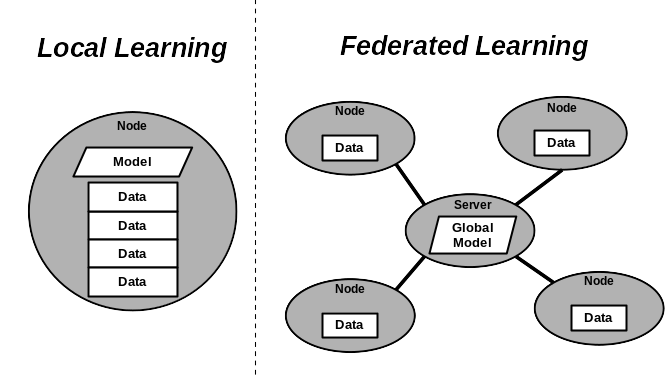
\includegraphics[width=\linewidth]{fed}
	\end{frame}

	\begin{frame}
		\frametitle{Federated Learning - Variations}
		\begin{itemize}
			\item Many variations of federated learning
			\begin{itemize}
				\item One of the originals is \emph{Federated Averaging (FedAvg)}
				\item Many other algorithms are based off this
			\end{itemize}
		\end{itemize}
	\end{frame}

	\begin{frame}
		\frametitle{FedAvg - How Does It Work?}
		\begin{itemize}
			\item FedAvg has repeated training steps. Each step:
			\begin{enumerate}
				\item Server sends model to a set of nodes
				\item Nodes perform training on the model
				\item Nodes send their models back to server
				\item New model is the average (mean) of all nodes models
			\end{enumerate}
		\end{itemize}
	\end{frame}

	\begin{frame}
		\frametitle{FedAvg - Issues}
		\begin{itemize}
			\item Vulnerable to central server going down
			\item Requires that every node has direct access to the server
			\item Scalability issues with bottleneck
		\end{itemize}
	\end{frame}

	\section{Swarm Learning}

	\begin{frame}
		\frametitle{Swarm Learning}
		\begin{itemize}
			\item No central server/node
			\item Each node has a distinct model, called the \emph{local model}
			\begin{itemize}
				\item Must keep all local models similar to each other
			\end{itemize}
			\item Each node has its own dataset
			\begin{itemize}
				\item This dataset cannot be shared with any other nodes
			\end{itemize}
			\item The goal is to train all local models together using all available data
		\end{itemize}
	\end{frame}

	\begin{frame}
		\frametitle{Swarm Learning}
		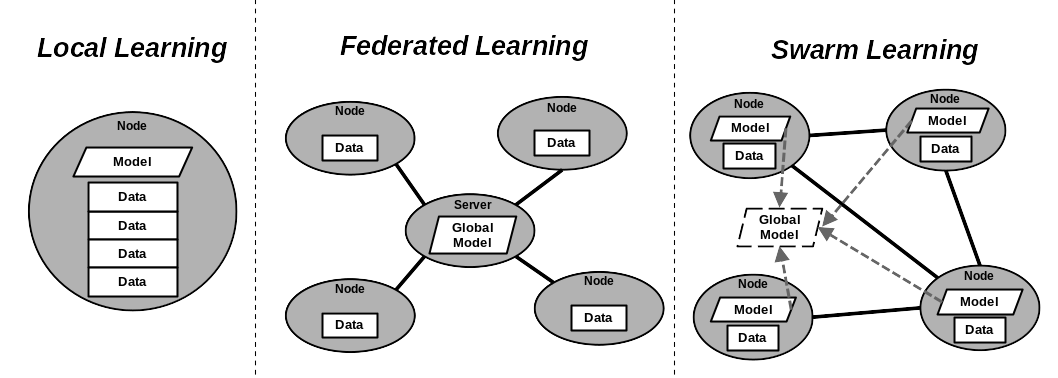
\includegraphics[width=\linewidth]{fedvsswarm}
	\end{frame}

	\begin{frame}
		\frametitle{SwarmAvg}
		\begin{itemize}
			\item SwarmAvg - \emph{Swarm Learning using Averaging}
			\item Inspired by FedAvg
			\begin{itemize}
				\item Model averaging is the core mechanic
			\end{itemize}
			\item No blockchain
			\item Local models of nodes are usually slightly different - no consensus on a global model
		\end{itemize}
	\end{frame}

	\begin{frame}
		\frametitle{SwarmAvg - How Does It Work?}
		\begin{itemize}
			\item Repeated Training Steps. Each node each step:
			\begin{enumerate}
				\item Perform training on the local model
				\item Send trained model to all neighbours
				\begin{itemize}
					\item This will get saved on the neighbour
				\end{itemize}
				\item New local model is the combination of all neighbours most recent local models
			\end{enumerate}
		\end{itemize}
	\end{frame}

	\begin{frame}
		\frametitle{SwarmAvg - Specifics}
		\begin{itemize}
			\item Different combination methods
			\begin{itemize}
				\item Combine by mean
				\item Combine with learning rate (weighted mean)
			\end{itemize}
			\item Only combine neighbours who have done more training than this node
			\item Wait for certain number of neighbours to catch up with this node
		\end{itemize}
	\end{frame}

	\begin{frame}
		\frametitle{Swarm Learning vs Issues of Federated Learning}
		\begin{itemize}
			\item \sout{Vulnerable to central server going down}
			\begin{itemize}
				\item No central server - to stop training you would have to take out every node
			\end{itemize}
			\item \sout{Requires that every node has direct access to the server}
			\begin{itemize}
				\item Swarm learning can function on sparse networks of nodes
			\end{itemize}
			\item \sout{Scalability issues with bottleneck}
			\begin{itemize}
				\item As the number of nodes in the network scales, the number of connections per node can stay consistent
			\end{itemize}
		\end{itemize}
	\end{frame}

	\section{Experiments}
	
	\begin{frame}
		\frametitle{What Did I Test?}
		Task was classification of MNIST fashion items, and results are accuracy of classification
		\begin{itemize}
			\item Tested SwarmAvg against FedAvg:
			\begin{itemize}
				\item In densely connected networks with varying amounts of available data
				\item In densely connected networks with varying amounts of available data and limited classes
			\end{itemize}
			\item Tested SwarmAvg:
			\begin{itemize}
				\item In sparsely connected networks with varying amounts of available data
				\item In sparsely connected networks with varying amounts of available data and limited classes
			\end{itemize}
		\end{itemize}
	\end{frame}

	\begin{frame}
		\frametitle{SwarmAvg Findings}
		\begin{itemize}
			\item In densely connected networks, SwarmAvg is slightly slower than FedAvg, and does not reach quite as high a final accuracy.
			\item With a high enough volume of data, SwarmAvg is only slightly affected by sparse network conditions, when no class restrictions are imposed.
			\item The effect of network sparsity on SwarmAvg is increased when class restrictions are introduced.
		\end{itemize}
	\end{frame}

	\begin{frame}
		\frametitle{Josh Pattman}
		Thanks for listening! Any questions?
	\end{frame}
	
\end{document}